\todo{Wichtige Begriffe erklären}
\subsection{Interferenz}
	\subsubsection{Verstärkung, Auslöschung, Weg- bzw. Phasenunterschied}
\subsection{Elektronen als Welle}
	\subsubsection{De Broglie Beziehung, Impuls, Wellenzahl usw.}
\subsection{Überlagerung von zwei Wellen}
	\subsubsection{Gleiche Wellen, entgegenlaufende Wellen, stehende Welle}
\subsection{Elektronen im Kastenpotential}
	\subsubsection{Einfacher Kasten, periodisches Kristallgitter}
\subsection{Bandstruktur von Halbleitern}
	\textbf{Bändermodell allgemein:}
	\begin{description}
		\item[Leitungsband:] Freie Elektronen (nicht mehr an ein bestimmtes Atom gebunden = Stromleitung möglich)
		\item[Bandlücke:] 'Verbotene Zone' $\rightarrow$ Energiebereich, ohne erlaubte Energieniveaus für Elektronen
		\item[Valenzband:] Energiebereich, in dem sich die äußeren Bindungselektronen des Atoms befinden (nicht für Stromleitung verfügbar) 
	\end{description}
	
	
	\subsubsection{Bandlücke, Brillouin-Zone
	Temperaturabhängigkeit}

		\textbf{Bandlücke bei Festkörpern:}
		\begin{description}
			\item[Metalle:] keine Bandlücke ($E_g$ = 0)
			\item[Isolatoren:] $E_g$ > 3eV
			\item[Halbleiter:] $E_g$ < 3eV
		\end{description}
		
		
\subsection{Direkte und indirekte Halbleiter}
	\begin{figure}[h!]
		\centering
		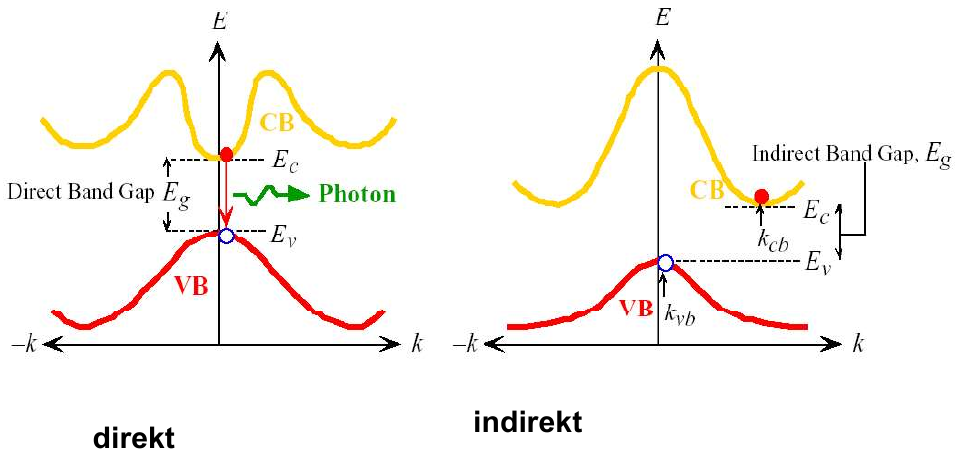
\includegraphics[width=\textwidth]{Kapitel/Kap03/uebergang_direkt_indirekt.png}
		\caption{direkter vs. indirekter Übergang}
		\label{02_uebergang}
	\end{figure}
	
	Für den Übergang von einem Elektron aus dem Valenzband ins Leitungsband ist bei einem direkten Halbleiter keine Impulsänderung notwendig; bei einem indirekten Halbleiter hingegen schon.
	
	\begin{figure}[h!]
		\centering
		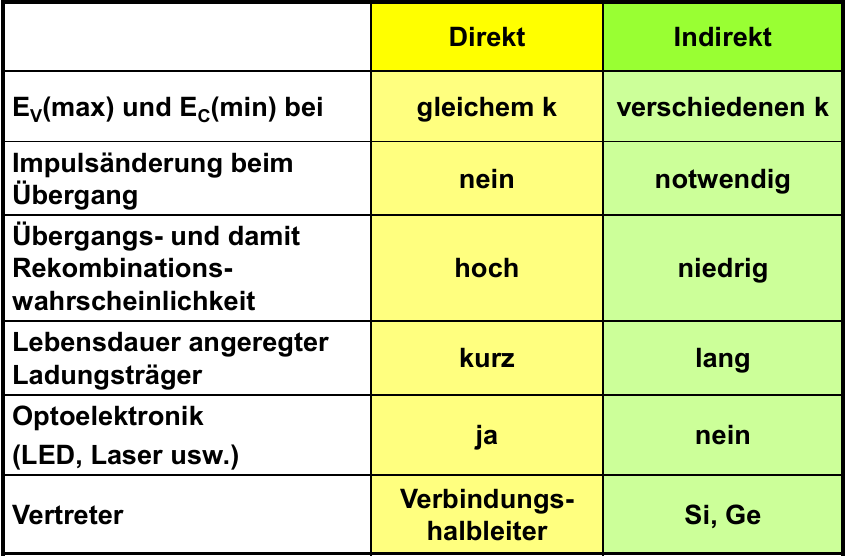
\includegraphics[width=0.8\textwidth]{Kapitel/Kap03/direkt_indirekt.png}
		\caption{direkter vs. indirekter Halbleiter}
		\label{02_dir_ind_hl}
	\end{figure}
	
\subsection{Effektive Massen}
	Es kann an den Minima und Maxima im Bändermodell unertschiedliche $E(k)$ -Funktionen geben, dies nennt man entartet. 
	Je flacher das Leitungsband am Minimum ist, desto schwerer wird die effektive Masse der Elektronen. Es gibt also 'schwere' und 'leichte' Massen (z.B. hh : heavy holes und lh: light holes), es können demnach auch heavy holes und light holes zusammen an den Maxima und Minima auftreten.
	Alle Massen tragen gewichtet nach ihren Anteilen zum Ladungstransport bei. 
	$\rightarrow$ analoges gilt auch für Löcher
	
	\begin{figure}[h!]
		\centering
		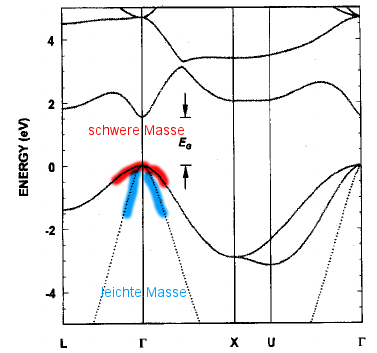
\includegraphics[width=0.3\textwidth]{Kapitel/Kap03/effektiveMasse.png}
		\caption{Beispiel: GaAs}
		\label{02_effMasse}
	\end{figure}

	Die Geschwindigkeit der Ladungsträger ist proportional zur elektrischen Feldstärke:
	\begin{equation*}
		v_n = {-\mu}_n E \quad \textrm{ und } \quad v_p = {\mu}_p E
	\end{equation*}
	
	Die Proportionalitätskonstante wird als \textbf{Beweglichkeit} bezeichnet. Wobei die Beweglichkeit mit steigender Masse abnimmt: ${\mu} \sim \frac{1}{m^*}$ ($m^* = effektive Masse$)
	Die Beweglichkeit von Löchern und Elektronen ist unterschiedlich.
	
\subsection{Verspanntes Silizium}
	Verpsannt man Silizium, so hebt man die Entartung auf. Die Ladungsträger werden so energetisch günstiger für den Transport.
	\begin{figure}[h!]
		\centering
		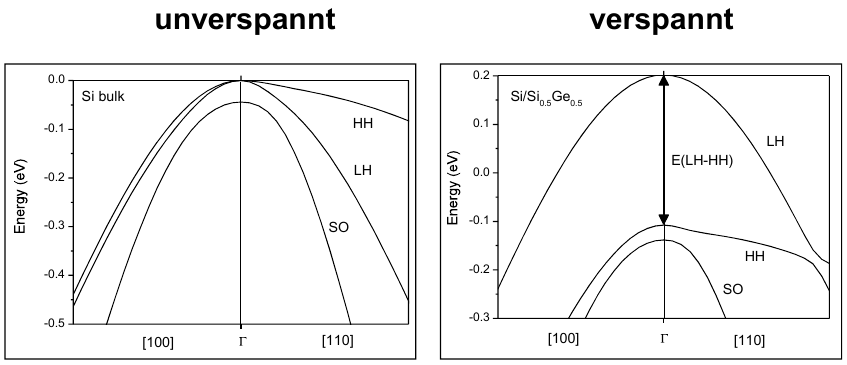
\includegraphics[width=0.5\textwidth]{Kapitel/Kap03/verspanntesSi.png}
		\caption{Spannungseinfluss im Valenzband (Silizium)}
		\label{02_verspSi}
	\end{figure}
	
\todo{Fragen aus Own Clowd zuordnen}
\todo{Gruppenübungs-Inhalte ergänzen}